\documentclass{article}
\usepackage{amsmath}
\usepackage{amssymb}
\usepackage{graphicx}
\usepackage{hyperref}
\usepackage[version=4]{mhchem}


\begin{document}
In right \(\triangle A B C, \angle B=90^{\circ}, \angle B A C=78^{\circ}\). Draw \(C F / / A B\). Connect \(A F\) and \(B C\). \(B C\) and \(A F\) meet at \(G\). If \(F G=2 A C\), find \(\angle B A G\).\\
\centering
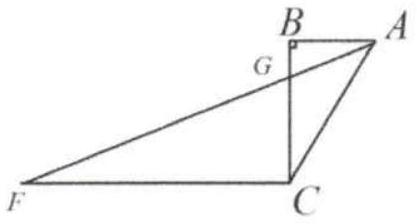
\includegraphics[width=\textwidth]{images/009(2).jpg}


Solution: \(26^{\circ}\).\\
Since \(A B / / C F, \angle F C B=90^{\circ} . \triangle F B C\) is a right triangle.\\
Take \(E\), the midpoint of \(F G\). Connect \(E C\).\\
\(E C=\frac{1}{2} F G=A C\).\\
Thus \(\angle E A C=\angle A E C=\angle F+\angle E C F=2 \angle F\).\\
Let \(\angle B A G=x . \angle F=x\).\\
\centering
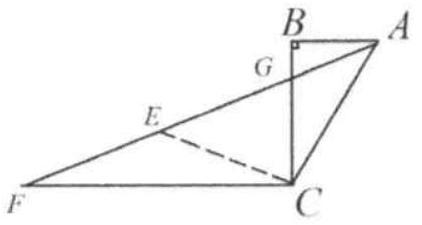
\includegraphics[width=\textwidth]{images/010(2).jpg}

So, \(x+2 x=78^{\circ} \quad \Rightarrow \quad x=26^{\circ}\).\\

\end{document}
